\documentclass[12pt]{article}


\usepackage[T1]{fontenc}
\usepackage[table]{xcolor}
\usepackage[title]{appendix}
\usepackage{mathtools,geometry,graphicx,empheq,wrapfig,upgreek,caption,subcaption,array,cleveref,IEEEtrantools}
\usepackage[numbered,framed]{matlab-prettifier}
\geometry{margin=0.75in, letterpaper}
\setlength\parindent{0pt}
\setlength{\arrayrulewidth}{1.5pt}
\newcolumntype{x}[1]{>{\centering\let\newline\\\arraybackslash\hspace{0pt}}m{#1}}
\newcolumntype{y}[1]{>{\centering\let\newline\\\arraybackslash\hspace{0pt}}p{#1}}
\graphicspath{{figures/}}

\bibliographystyle{ieeetr}

\title{\vspace{-1cm}Design Proposal - Student Challenge ASPE 2019}
\date{}
\author{UNC Charlotte\\ Kumar Arumugam, Alexander Blum, Kristen Venditti, Jacob Cole\\ Supervisor: Dr. Joshua Tarbutton}




\begin{document}
\maketitle

\section{Introduction}

This document describes a device which uses the Watt balance principle to estimate the mass of unknown samples and report the uncertainty in measurement.


\section{Design Overview}

Figure 1 shows the design of a mass measuring device that includes an axially translated stage in the z-direction. The translating mechanism consists of a double compound rectilinear flexure \cite{smith2000} chosen for its single degree of freedom in motion. Each link shown in green is a stack of 4 leaves bolted together to increase the stiffness of the mechanism. Two voice coils are attached to the top (coil A) and bottom (coil B) of the moving stage and the magnets are held concentrically to the coils on the upper and lower frames. 

\begin{figure}[ht!]
	\centering
	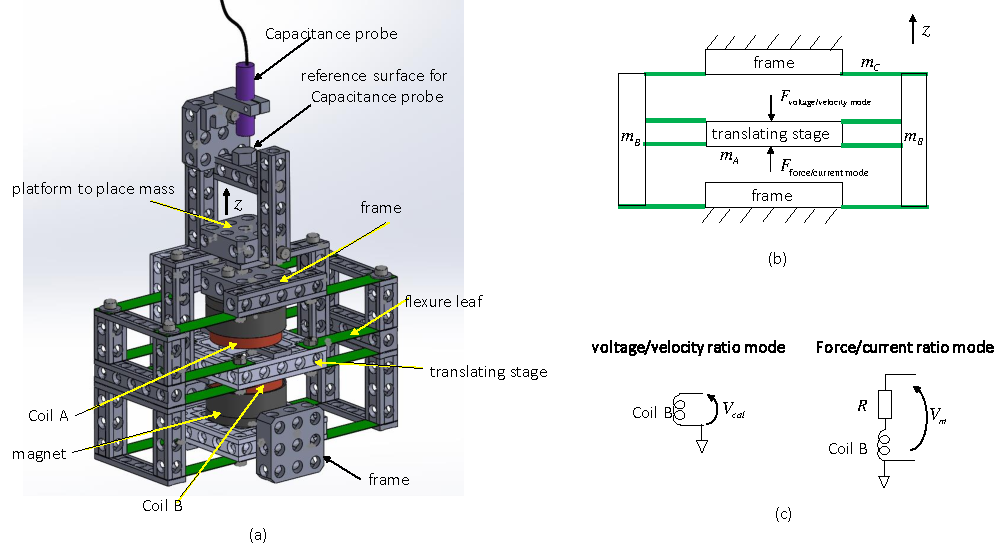
\includegraphics[height = 3.7in]{fig1}
	\caption{Solid model (a) and schematic (b) of the mass measuring device consisting of a double compound rectilinear flexure. During the mass measurement, this flexure is actuated by coil B at a known force to oppose the gravitational pull of an unknown mass. Circuit diagrams (c) show the potential differences measured across coil B in the two modes of operation to estimate the mass.}
	\label{fig:1}
\end{figure}
\pagebreak

\section{Experiments}

There are two experiments employing the following equations that must be performed to measure an unknown mass.

\subsection{Experiment 1: Voltage / Velocity Mode}

From \cite{chao2015},
\begin{equation}
	V_{cal} = BLv.
\end{equation}
To assess the force sensitivity of current ($BL$) in coil B, the stage is oscillated using coil A at a velocity ($v$). This induces an electromagnetic force ($V_{cal}$) in coil B, which is measured across the coil. Velocity ($v$) is computed from the displacement ($z$) measured using a capacitance probe placed axially to the moving stage, see Figure \ref{fig:1}, and the time ($t$) obtained from the internal clock of the microprocessor (NI myRIO).

\subsection{Experiment 2: Force / Current Mode}\label{sec:experiment2}

From \cite{chao2015},
\begin{equation}
	mg = BLI.
\end{equation}
When an object whose mass ($m$) is to be measured is placed on the stage, the stage sinks down. Coil B, whose $BL$ is estimated in the velocity mode experiment above, is energized to bring the stage back to its initial position. The current that is utilized for this process is calculated by the voltage ($V_m$) measured across a sense resistor ($R$), see Figure \ref{fig:1}. The sense resistor is situated in the amplification circuit to drive coil $B$ and is connected in series with it.

Therefore, the estimated mass of the object is, 
\begin{equation}
	m = \frac{V_{cal}V_m}{vRg}.
\end{equation}
	
\subsection{Sanity Check}

As a sanity check to validate the value of $BL$, Experiment 2 is performed with a reference mass ($m_{ref}$) and the current ($I$) to take the stage to its initial position is measured. Force sensitivity is given by 
\begin{equation}
BL = \frac{m_{ref}g}I.
\end{equation}

\section{System Characteristics}

System characteristics tabulated in Table \ref{tab:1} show that the theoretically calculated, undamped resonant frequency is $f_{n,theory}$ = 23 Hz, and that the stiffness is $k_{theory}$ = 10924 N/m. Whereas, an experiment performed with a Dynamic Signal Analyzer (DSA, Hewlett Packard 35665A) shows that the fundamental resonant frequency is at 25 Hz, see Figure \ref{fig:2}. From Equation \ref{eq:fntheory} in Table \ref{tab:1}, for $f_{n,DSA}$ = 25 Hz, stiffness is calculated to be $k_{DSA}$ = 12300 N/m. 

To experimentally validate the true stiffness of the system, two known masses of 33 g and 52 g were placed on the moving platform, for which the resulted sag recorded by the cap probe was 0.11 mm and 0.17 mm respectively. This estimates that the stiffness of the system is approximately 3000 N/m. 

A flexure link consisting of four leaves bolted together may behave different to a single leaf of equivalent thickness. This may cause the stiffness of the system to vary from the theoretical prediction.

Though the stiffness values from above estimations differ, resonant frequency ($f_{n,DSA}$ = 25 Hz) validated using the DSA implies that the maximum achievable velocity in Voltage / Velocity mode is $A\omega = 2\pi{}Af_{n,DSA}$ = 0.04 m/s, where, $A$ = 0.25 mm is the maximum amplitude of sinusoidal displacement measurable by the capacitance probe.

\begin{table}[ht!]
\centering
	\begin{tabular}{x{26mm} x{54mm} x{50 mm} x{23mm}}
		\hline
		\textbf{Quantity} & \textbf{Formula} & \textbf{Parameter} & \textbf{Value}\\
		\hline
		\textbf{Mobility} & $M = 3(n-j-1)+f$ &number of links, $n=4$\newline{}number of joints, $j=8$\newline{}degrees of freedom,\newline{}$f = 2j = 16$\newline& 1\\
		\textbf{Stiffness} & $k_{theory}=8\frac{12Ebt^3}{l^2}$ & $b=12.7$ mm; $t=0.3$ mm;\newline $l=37.5$ mm; $E=210$ GPa & 10924 Nm$^{-1}$\\
		\textbf{Undamped\newline{}Resonant\newline{}Frequency} & \begin{flalign}
		f_{n,theory}=\tfrac{1}{2\pi}\sqrt{\tfrac{2k}{M_A+\tfrac{1}2M_B}}\label{eq:fntheory}\end{flalign}& $M_A=0.370$ kg\newline $M_B=0.280$ kg\newline (See Figure \ref{fig:1}) & 23 Hz\\
		\textbf{Max Force\newline{}Provided by\newline{}Voice Coil\newline} & $F_{max} = BLI_{max}$ & $BL = 13.2$ N/A \cite{hardwaremanual}\newline{}Max current from amplifier,\newline{}$I_{max}=\pm1$ A & $\pm13.2$ N\\
		\textbf{Max\newline{}Displacement} & $z_{max}=\frac{F_{max}}{k_{theory}}$ & & $\pm1.2$ mm\\
		\hline
	\end{tabular}
	\caption{System characteristics \cite{smith2000}}
	\label{tab:1}
\end{table}

\begin{figure}[ht!]
	\centering
	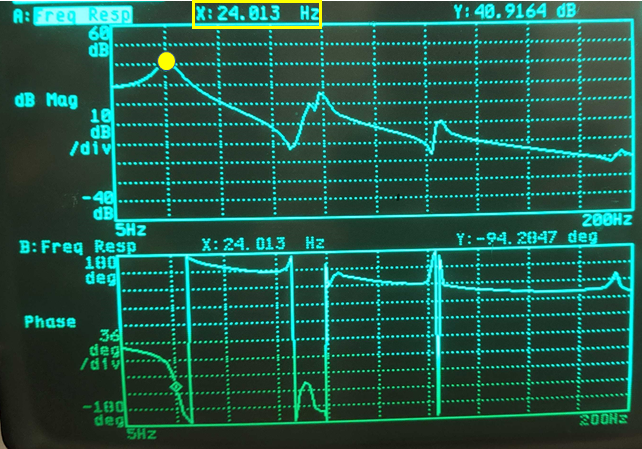
\includegraphics[width=0.55\linewidth]{fig2}
	\caption{Experimental result showing that the fundamental resonant frequency of  the system is 25 Hz.}
	\label{fig:2}
\end{figure}

\subsection{Actuator Considerations}
\subsubsection{Physical Interference of Coil and Magnet}
From Table \ref{tab:1}, the travel range of the stage ($z_{max}= \pm 1.2$ mm) is limited by the current,  $I_{max}=\pm1$ A, that could be supplied to the coil. This travel range is less than the stroke length $\pm3$ mm \cite{hardwaremanual} of the voice coil. Therefore, the coil would not physically touch the magnet during its motion.  
\subsubsection{Sag of the Stage Due to Its Own Mass and Sample Mass}
From Table \ref{tab:1}, for $k_{theory}= 10924$ N/m, mass of the translating stage ($m_A  = 0.37$ kg) would cause a sag of $z_{sag}= - 0.33$ mm. The maximum mass of an unknown sample provided in the challenge is around $m_{max}= 0.4$ kg. This would cause an additional sag of $- 0.35$ mm.  Since the total displacement of $- 0.88$ mm is within the travel range of the stage ($z_{max}= \pm 1.2$ mm), the stage could be controlled to its zero position during Force / Current Mode (see Section \ref{sec:experiment2}).

\section{Sensor Choice}
\subsection{Capacitance Probe}
In Voltage / Velocity Mode, for an undamped system with a resonant frequency of $f_n = 25$ Hz, and the travel range of the cap probe $z_{max,cp}=0.5$ mm, the maximum achievable velocity of the stage is $v_{max}= 0.04$ m/s.

In current mode, since the stage’s position can be zeroed via the PID controller, the limited $z_{max,cp}$ of the capacitance probe is not relevant. 
\subsection{Knife Edge Sensor}
In Voltage / Velocity Mode, for an undamped system with a resonant frequency of 25 Hz, if one chose to use the linear range (0.1 mm) of a knife edge sensor (RPI0352E) with a flat blade, the maximum velocity of stage motion is 0.008 m/s. The corresponding induced emf ($V_{cal}$) would be less compared to using the capacitance probe’s 0.5 mm range. Using an angled blade with a knife edge sensor could provide a measurable range of 1.64 mm, however, the voltage output is non-linear as most of the intensity is concentrated at the center of the Gaussian beam profile. Therefore, a look up table could be used for correcting the non-linearity.

Considering the advantage of the sensitivity of $V_{cal}$  to velocity ($v$), and ease of use, a capacitance probe was chosen as the sensor.

\section{Control Architecture and Signal Conditioning}
\subsection{Voltage / Velocity Mode}
Velocity mode follows an open loop control architecture where coil A is actuated using a sinusoidal voltage input. After applying a moving average filter on the displacement measured by the capacitance probe, the velocity of the stage motion is calculated. 
\begin{figure}[ht!]
	\centering
	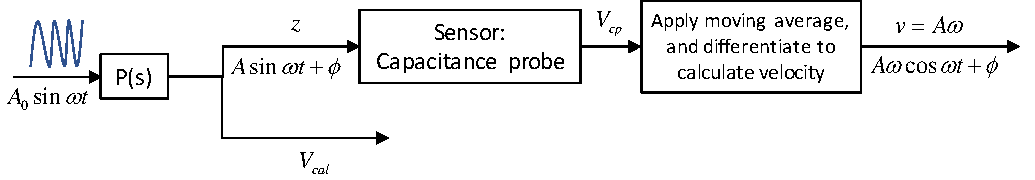
\includegraphics[height=1.2in]{open-loop}
	\caption{Control architecture using an open loop system in Voltage / Velocity Mode.}
	\label{fig:open-loop}
\end{figure}
\subsection{Force / Current Mode}
A PID controller is utilized to keep the stage at its initial position using the feedback from the capacitance probe. When a mass is placed on the stage, the current required to keep the stage at the initial position increases. This current is computed by measuring the voltage ($V_m$) across the sense resistor, see Figure \ref{fig:1}.
\begin{figure}[ht!]
	\centering
	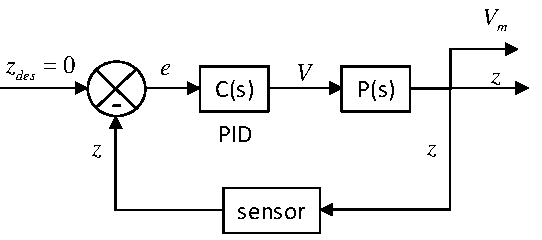
\includegraphics[height=1.6in]{closed-loop}
	\caption{Control architecture using a closed loop PID controller in Force / Current Mode}
	\label{fig:closed-loop}
\end{figure}

\section{Uncertainty Analysis}
\subsection{Uncorrelated quantities contributing to standard uncertainties in measurement \cite{gum2008}}
Estimated mass of the object,
\begin{equation}
m = \frac{V_{cal}V_m}{vRg} = f(V_{cal},V_m,v,R,g).
\end{equation}
Assuming input quantities are uncorrelated, combined uncertainty in the measurement of mass ($\delta_m$) is expressed as
\begin{IEEEeqnarray}{rCl}\label{eq:5}
	{\delta_m}^2 & = & \left(\frac{\partial m}{\partial V_{cal}}\right)^2{\delta_{V_{cal}}}^2 + \left(\frac{\partial m}{\partial V_{m}}\right)^2{\delta_{V_{m}}}^2 + \left(\frac{\partial m}{\partial R}\right)^2{\delta_{R}}^2 + \left(\frac{\partial m}{\partial A\omega}\right)^2{\delta_{A\omega}}^2 + \left(\frac{\partial m}{\partial g}\right)^2{\delta_{g}}^2\\
	& = & \left(\frac{V_m}{vRg}\right)^2{\delta_{V_{cal}}}^2 + \left(\frac{V_{cal}}{vRg}\right)^2{\delta_{V_{m}}}^2 + \left(-\frac{V_{cal}V_m}{vR^2g}\right)^2{\delta_{R}}^2 + \left(-\frac{V_{cal}V_m}{v^2Rg}\right)^2{\delta_{A\omega}}^2 + \left(-\frac{V_{cal}V_m}{vRg^2}\right)^2{\delta_{g}}^2\nonumber
\end{IEEEeqnarray}
The combined uncertainty in measurement of the mass is $\delta_m = \pm 0.8$ g. $$ \textrm{Mass,}m=m_{nominal}\pm0.8\textrm{ g (}k=1\textrm{)} $$

Tables \ref{tab:2} and \ref{tab:3} show the values of the nominal quantities and standard uncertainties used in Equation \ref{eq:5}.

\begin{table}[ht!]
\centering
	\begin{tabular}{x{36mm} x{44mm} x{50 mm} x{23mm}}
		\hline
		\textbf{Quantity} & \textbf{Formula} & \textbf{Parameter} & \textbf{Value}\\
		\hline
		\multicolumn{4}{c}{\cellcolor{gray!40}\textit{Voltage / Velocity Mode}}\\
		\textbf{Maximum\newline{}Achievable\newline{}Velocity} & $v=A\omega=A(2\pi{f})$ &Frequency of Oscillation, $f=25$ Hz\newline{}$A=\tfrac{1}2z_{max,cp}=0.25$ mm\newline& 0.04 m/s\\
		\textbf{Induced EMF} & $V_{cal}=BLv$ & $BL=13.2$ N/A \cite{hardwaremanual} & 0.1 V\\
		\multicolumn{4}{c}{\cellcolor{gray!40}\textit{Force / Current Mode}}\\
		\textbf{Voltage\newline{}Measured\newline{}Across Resistor} &$V_m=\frac{mgR}{BL}$&$m=0.4$ kg\newline{}$R=2.2\,\Omega$& 0.66 V\\
		\hline
	\end{tabular}
	\caption{Values of nominal  quantities used in the uncertainty expression (Equation \ref{eq:5}).}
	\label{tab:2}
\end{table}

\begin{table}[ht!]
\centering
	\begin{tabular}{x{35mm} x{31mm} x{60mm} x{36mm}}
		\hline
		\textbf{Std. Uncertainty\newline{}Component} & \textbf{Symbol} & \textbf{Parameter} & \textbf{Value}\\
		\hline
		\textbf{Acceleration Due\newline{}To Gravity\newline} & $\delta_g$ &  & $3\times10^{-5}$ m/s$^2$ \cite{ngs,mapcoords}\\
		\textbf{Induced EMF in\newline{}V/$v$ Mode\newline} & $\delta_{V_{cal}}=\frac{V_{range,ADC}}{2^{nb}-1}$\newline & $V_{range,ADC}=\pm10$ V\newline{}$nb=14$ bits\newline{}(2 bits of noise in a 16-bit ADC)\newline & 0.6 mV\newline \\
		\textbf{Voltage Across\newline{}Resistor in\newline{}$F$/$I$ Mode\newline} & $\delta_{V_m}=\frac{V_{range,ADC}}{2^{nb}-1}$\newline &  & 0.6 mV\newline\\
		\textbf{Resistance of\newline{}Sense Resistor} &$\delta_R$&& 1 m$\Omega$ \cite{ampmanual}\\
		\textbf{Velocity} &$\delta_v=\omega\delta_A+A\delta_\omega$& \newline{}resolution of displacement\newline{}measured by capacitance probe,\newline{}$\delta_A=30$ nm\newline{}$\,$\newline{}resolution of frequency of\newline{}oscillation,\newline{}$\delta_\omega=-\frac{2\pi{f}\delta_t}t=0.94$ mrad/s\newline{}$\,$\newline{}resolution of time in MyRIO's\newline{}clock, $\delta_t=6\,\upmu$s\newline{}(resolution of quartz oscillator is\newline{}6 ppm)& $1.9\times10^{-7}$ m/s\\		
		\hline
	\end{tabular}
	\caption{Values of standard uncertainties used  in the uncertainty expression (Equation \ref{eq:5}).}
	\label{tab:3}
\end{table}

\subsection{Contributors to Uncertainty in Measurement: Temperature, Pressure and Humidity}\label{sec:7.2}
\begin{figure}[ht!]
	\centering
	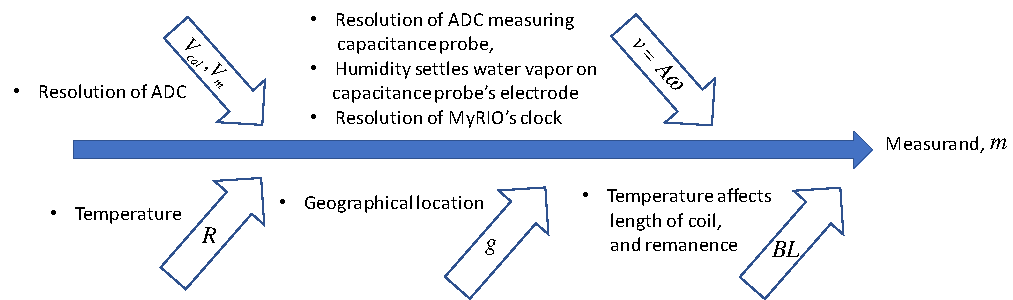
\includegraphics[height=2in]{fishbone}
	\caption{Fishbone diagram showing the factors affecting input quantities.}
	\label{fig:fishbone}
\end{figure}
\subsubsection{Capacitance Probe}
Variation in the capacitance probe reading could be caused by tilt of the probe with target surface, surface roughness, atmospheric temperature, pressure and more dramatically by humidity \cite{harmsen2010}. For a probe with 50 $\upmu$m electrode spacing, the distance measured could vary up to 825 nm in 100 minutes. Considering the experiments in both velocity and current mode are performed in roughly 1 minute, the variation in displacement would be less than 10 nm; this is less than $\delta_A=30$ nm.
\subsubsection{Resistance of the Sense Resistor}
Resistance of the sense resistor changes with temperature and will be taken into consideration when the temperature dependence data is made available by the Challenge Committee. 
\subsubsection{Length of the Coils}
The length of the coil ($L$) increases with the temperature and affects both force sensitivity ($BL$) and resistance of the coil, $R=\frac{\rho{L}}A$. The information of $L$ and $A$ are not given in the hardware sheet and our efforts to approximate did not yield the given resistance, $R=8.58\,\Omega$.
\subsubsection{Remanence}
Assuming a temperature change in the facility of $\pm2\,^\circ\textrm{C}$, magnetic flux ($B$, remanence) of a Neodymium Iron Boron (NdFeB) magnet would vary $\approx0.2 \%$ \cite{ndmagnets} in between two modes of operation.

This could cause an uncertainty of $\delta_m=0.8$ g in measuring a 400 g mass.
\subsubsection{Mass}
Considering the humidity in the atmosphere deposits a 10 nm layer of water on the surface area of mass \cite{harmsen2010}, an additional 60 ng will be added to the true mass. This is negligible compared to other contributors of uncertainty. 
\subsubsection{Sensitive Term}
The most sensitive term in the expression of uncertainty (Equation \ref{eq:fntheory}) is the maximum achievable velocity, $v=A\omega$.

\subsection{Monte Carlo Simulation}
For a more rigorous uncertainty estimate, a Monte Carlo simulation was performed for one million iterations (see Appendix). Each uncertainty term was considered as normally distributed. The resulted histogram shows a conservative estimate of standard deviation, $\sigma_{x_i}=10$ g in a single measurement. For a repeated measurement of the same sample mass $n=10$ times , standard deviation was $\sigma_{x_i}=\frac{\sigma_{x_i}}{\sqrt{n}}=3.2$ g. 

\begin{figure}[ht!]
	\centering
	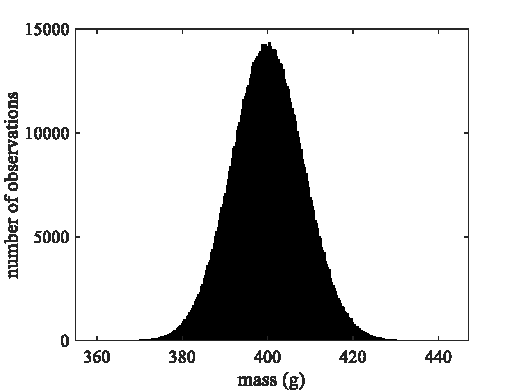
\includegraphics[height = 2.6in]{histogram}
	\caption{Result of one million simulated measurements of a nominal mass of 400 g.}
	\label{fig:histogram}
\end{figure}

There is  disagreement between Monte Carlo simulation and the calculation using derivatives (see Section \ref{sec:7.2}). To experimentally validate the uncertainty in measurements, repeated mass measurements will be performed and the standard deviation will be computed during the construction phase. 

\section{Conclusion}
Design of a mass measuring device using a watt balance principle is described. This design is novel, and does not follow any of the Watt balances designed and built by national standards laboratories. The mechanism conserves symmetry in actuation and displacement measurement, avoiding Abbe errors. The stage mechanism could be actuated at a maximum velocity of $v_{max}= 0.04$ m/s.

Control architecture followed in two modes of operation to estimate the mass of an unknown sample is described.

Uncertainty of the measurement of mass is estimated using derivative method and Monte Carlo simulation. The disagreement between the methods will be evaluated experimentally during the construction phase.

$$m_{derivative method}=m_{nominal}\pm0.8\textrm{ g (}k=1\textrm{)}$$
$$m_{Monte Carlo}=m_{nominal}\pm10\textrm{ g (}k=1\textrm{)}$$

\bibliography{references}
\pagebreak


\section{Bill of Materials}

\center{\textit{Highlighted in yellow are the $\mathbf{4}$ additional components of choice.}}

\begin{table}[ht!]
	\centering
	\begin{tabular}{p{0.3\textwidth} x{0.10\textwidth}}
		\hline
		\multicolumn{2}{c}{\textbf{MechBlock Components}}\\
		\hline
		\cellcolor{gray!40}Part& \cellcolor{gray!40}Qty\\
		B11-5-5-N		& 6		\\
		B11-3-3-N		& 3		\\
		B11-5-1-N		& 8		\\
		\cellcolor{yellow!40}B11-3-1-N		& \cellcolor{yellow!40}4		\\
		\cellcolor{yellow!40}B11-2-1-N		& \cellcolor{yellow!40}4		\\
		B11-1-1-N		& 0		\\
		\cellcolor{yellow!40}B10-5-0.25-EC	& \cellcolor{yellow!40}10		\\
		B10-1-0.25-EC	& 8		\\
		C11-1.5-9.5-N	& 1		\\
		CP10-1-0.5-FL	& 1		\\
		\hline\\
	\end{tabular}
	\caption{Mech blocks used in the construction of the mass measuring device (highlighted are the 4 additional components of choice).}
\end{table}



Mailing Address: \\
\begin{center}
Center for Precision Metrology\\
Duke Centennial Hall 108C\\
University of North Carolina at Charlotte \\
9201 University City Boulevard\\
Charlotte, NC  28223
\end{center}
Phone Number: 
\begin{center}
(704) 906-6813  (Kumar)
\end{center}
\pagebreak

\begin{appendices}
\section{}
Program to perform a Monte Carlo simulation to predict the uncertainty in the measurement of mass

\lstinputlisting[style=Matlab-editor]{montecarloprogram.m}

\end{appendices}
\end{document}





